\chapter{User Guide}\label{ch:user-guide}

This book template provides a \LaTeX\ style for use in National 
University of Singapore (NUS) theses
and qualifying-examination (QE) reports. This is \emph{not}
an official template provided by NUS (this is experimental and
may not be approved by NUS). This chapter is a guide to
the processing of preparing your thesis/report for submission.
Subsequent chapters (\cref{ch:cat,ch:concl} and \cref{app:moduli})
are sample gibberish.

The \texttt{nusthesis-neo} document class can be used to prepare
both theses and QE reports, both for print and electronic submissions,
and for any stage of submission, from review to final ``camera-ready''
copy, with \emph{very} few changes to the source.

\section{Template Options}\label{sec:template-options}

The \texttt{nusthesis-neo} document class is extended from the \texttt{memoir}
document class.\footnote{\url{https://ctan.org/pkg/memoir?lang=en}} 
As such, configuration options for \texttt{memoir} are also applicable to
\texttt{nusthesis-neo}.

\texttt{\textbackslash documentclass[OPTIONS]\{nusthesis-neo\}}

The \texttt{nusthesis-neo} class exposes additional configuration parameters:
\begin{enumerate}
    \item \texttt{qe}: configure this document to be a QE report
    \item \texttt{review}: enable line numbers for reviewing
    \item \texttt{twoside}: two-sided formatting for printing purposes
    (should not be used for final electronic submission)
    \item \texttt{print}: disable coloring for printing purposes
    \item \texttt{numcite}: use numeric citations (see \cref{sec:citations})
\end{enumerate}

For example, to use the \texttt{qe} and \texttt{review} options, use the
following \texttt{documentclass} header:

\texttt{\textbackslash documentclass[qe,review]\{nusthesis-neo\}}

To conditionally define or insert things in the document if \texttt{print}
mode is enabled/disabled, you may use the \texttt{printonly}/\texttt{screenonly} 
environments, respectively. The following paragraph is
different in the rendered document depending on whether \texttt{print}
is enabled in the document class options.

\begin{printonly}
This paragraph appears only in the print version of the paper.
You can use this environment to set colors to grayscale, insert
b\&w images, etc.
\end{printonly}

\begin{screenonly}
This paragraph appears only in the screen (no \texttt{print}) version of the paper.
You can use this environment to define colors, insert colored
images, etc.
\end{screenonly}

\section{Typefaces}\label{sec:typefaces}

The \texttt{nusthesis-neo} document class requires the use of \texttt{helvet},
\texttt{newtxtext}, \texttt{newtxmath} and \texttt{inconsolata} font
packages.
Your \TeX\ installation should include
this set of packages. Please do not substitute other typefaces. The
``\verb|lmodern|'' and ``\verb|ltimes|'' packages should not be used,
as they will override the built-in typeface families.

\section{Abstract Name}\label{sec:abstract-name}
By default, the name of the abstract is ``Abstract''. However, the
Graduate Division may require the name to be ``Summary''. To change
this name, issue the command \texttt{\textbackslash changeabstractname}
and set it to ``Summary'', or whichever name is required.

\texttt{\textbackslash changeabstractname\{Summary\}}

\section{Title Information}\label{sec:title}

The title of your work, and the titles of all headings (chapters,
sections, etc.) should use capital letters appropriately---\url{https://capitalizemytitle.com/}
has useful rules for capitalization. Use the \texttt{title} command to define the title of
your work. 

\section{Author, Advisor(s) and Examiner(s)}

Write your name in the \texttt{author} command:

\texttt{\textbackslash author\{Your Name\}}

You may optionally include your previous degrees; each degree can be included with the \texttt{\textbackslash prevdegree} command:

\texttt{\textbackslash prevdegree\{B.A., National University of Singapore\}}

\texttt{\textbackslash prevdegree\{M.S., Nanyang Technological University\}}

Set the degree, field of study and the year of the \emph{first submission} of the thesis.

\texttt{\textbackslash degree\{Doctor of Philosophy\}}

\texttt{\textbackslash field\{Computer Science\}}

\texttt{\textbackslash degreeyear\{2028\}}

Include your advisor(s) in the cover page. Each advisor is included
via the \texttt{\textbackslash advisor} command. Multiple advisors
are permitted.

\texttt{\textbackslash advisor\{Professor X\}}

\texttt{\textbackslash advisor\{Professor Y\}}

\texttt{\textbackslash advisor\{Professor Z\}}

Examiners can also be included in the cover page. Each examiner
is defined using the \texttt{examiner}
command. You should omit examiners until the final submission.

\texttt{\textbackslash examiner\{Professor A\}}

\texttt{\textbackslash examiner\{Professor B\}}


\section{Declaration}

NUS theses require a declaration, which can be configured using the
\texttt{declaredate} and \texttt{declaresign} commands. If you prefer
to sign physically, the \texttt{declaresign} command can be omitted.

\texttt{\textbackslash declaredate\{1 Jan 2028\}}

\texttt{\textbackslash declaresign\{pic/signature.png\}}

Once your declaration page has been configured, you can create the
declaration page using \texttt{\textbackslash declarationpage}.

\section{Front Matter}

The front matter has been typeset for you in the \texttt{frontmatter}
environment (see \texttt{main.tex}). Change the content of:
\begin{itemize}
    \item The dedication (\texttt{\textbackslash dedicate\{...\}})
    \item The acknowledgements (\texttt{\textbackslash begin\{acknowledgments\}...\textbackslash end\{acknowledgments\}})
    \item The abstract (\texttt{\textbackslash begin\{abstract\}...\textbackslash end\{abstract\}})
\end{itemize}
The table of contents (\texttt{\textbackslash tableofcontents}), list of tables
(\texttt{\textbackslash listoftables}) and list of figures (\texttt{\textbackslash listoffigures})
can be omitted if preferred, especially if your report does not have tables/figures. Avoid
configuring the other settings in the front matter.

\section{Sectioning Commands}

Your work should use standard \LaTeX\ sectioning commands:
\verb|\chapter|, \verb|\section|, \verb|\subsection|, \verb|\subsubsection|,
\verb|\paragraph|, and \verb|\subparagraph|. The sectioning levels up to
\verb|\subsubsection| should be numbered; do not remove the numbering
from the commands. Appendices should be placed after the \verb|\appendix|
command.

Below are examples of sectioning commands.

\subsection{Subsection}
\label{sec:subsection}

This is a subsection.

\subsubsection{Subsubsection}
\label{sec:subsubsection}

This is a subsubsection.

\paragraph{Paragraph}

This is a paragraph.

\subparagraph{Subparagraph}

This is a subparagraph.

\section{Tables}

The \texttt{memoir} (and thus \texttt{nusthesis-neo}) document class includes the
\texttt{booktabs} package\footnote{\url{https://ctan.org/pkg/booktabs}} for preparing
high-quality tables. Table captions are placed {\itshape above} the table.

Because tables cannot be split across pages, the best placement for
them is typically the top of the page nearest their initial cite.  To
ensure this proper ``floating'' placement of tables, use the
environment \texttt{table} to enclose the table's contents and the
table caption.  The contents of the table itself must go in the
\texttt{tabular} environment, to be aligned properly in rows and
columns, with the desired horizontal and vertical rules.  Again,
detailed instructions on \texttt{tabular} material are found in the
\textit{\LaTeX\ User's Guide}.

Immediately following this sentence is the point at which
\cref{tab:freq} is included in the input file; compare the
placement of the table here with the table in the printed output of
this document.

\begin{table}
  \caption{Frequency of Special Characters}
  \label{tab:freq}
  \centering
  \begin{tabular}{ccl}
    \toprule
    Non-English or Math&Frequency&Comments\\
    \midrule
    \O & 1 in 1,000& For Swedish names\\
    $\pi$ & 1 in 5& Common in math\\
    \$ & 4 in 5 & Used in business\\
    $\Psi^2_1$ & 1 in 40,000& Unexplained usage\\
  \bottomrule
\end{tabular}
\end{table}

Always use midrule to separate table header rows from data rows, and
use it only for this purpose. This enables assistive technologies to
recognise table headers and support their users in navigating tables
more easily.

\section{Math Equations}
You may want to display math equations in three distinct styles:
inline, numbered or non-numbered display.  Each of the three are
discussed in the next sections.

\subsection{Inline (In-text) Equations}
A formula that appears in the running text is called an inline or
in-text formula.  It is produced by the \texttt{math} environment,
which can be invoked with the usual
\texttt{{\char'134}begin\,\ldots{\char'134}end} construction or with
the short form \texttt{\$\,\ldots\$}. You can use any of the symbols
and structures, from $\alpha$ to $\omega$, available in
\LaTeX~\parencite{Lamport:LaTeX}; this section will simply show a few
examples of in-text equations in context. Notice how this equation:
\begin{math}
  \lim_{n\rightarrow \infty}x=0
\end{math},
set here in in-line math style, looks slightly different when
set in display style.  (See next section).

\subsection{Display Equations}
A numbered display equation---one set off by vertical space from the
text and centered horizontally---is produced by the \texttt{equation}
environment. An unnumbered display equation is produced by the
\texttt{displaymath} environment.

Again, in either environment, you can use any of the symbols and
structures available in \LaTeX\@; this section will just give a couple
of examples of display equations in context.  First, consider the
equation, shown as an inline equation above:
\begin{equation}
  \lim_{n\rightarrow \infty}x=0
\end{equation}
Notice how it is formatted somewhat differently in
the \texttt{displaymath}
environment.  Now, we'll enter an unnumbered equation:
\begin{displaymath}
  \sum_{i=0}^{\infty} x + 1
\end{displaymath}
and follow it with another numbered equation:
\begin{equation}
  \sum_{i=0}^{\infty}x_i=\int_{0}^{\pi+2} f
\end{equation}
just to demonstrate \LaTeX's able handling of numbering.

You may also use the \texttt{align} environment for aligning
multi-line equations:
\begin{align}
    \label{eq:123}
    1 + 2 + 3 &= 3 + 3\\
    \label{eq:33}
    &= 6
\end{align}

\subsection{Theorem Environments}
The \texttt{nusthesis-neo} document class uses \texttt{tcolorbox} to typeset
theorem environments. There are many kinds of theorem-like environments
available: \texttt{theorem}, \texttt{lemma}, \texttt{corollary},
\texttt{proposition}, \texttt{conjecture}, \texttt{axiom}, \texttt{definition},
\texttt{example} and \texttt{remark}. These environments have two arguments.
The first argument is an optional description of the environment. The
second argument is the label for the theorem. Note that labels are
prepended with a short string describing the environment. These labels are:
\texttt{thm:} (\texttt{theorem}), \texttt{lem:} (\texttt{lemma}),
\texttt{cor:} (\texttt{corollary}),
\texttt{prop:} (\texttt{proposition}), 
\texttt{conj:} (\texttt{conjecture}), 
\texttt{ax:} (\texttt{axiom}),
\texttt{def:} (\texttt{definition}),
\texttt{eg:} (\texttt{example}) and \texttt{rem:} (\texttt{remark}).
Additionally, a \texttt{proof} environment is provided, and an optional
argument can be provided to customize the title of the proof. Examples
are given below:

\begin{definition}{}{no-name}
This definition has no name.
\end{definition}

\begin{lemma}{Named Lemma}{named}
This lemma has a name.
\end{lemma}

\begin{proof}[Proof Sketch]
Based on this incredibly obvious identity:
\[1 + 1 = 3\]
The proof is immediate.
\end{proof}

The labels used for references are Definition~\ref{def:no-name} and Lemma~\ref{lem:named},
respectively.

\section{Figures}

The \verb|figure| environment should be used for figures. One or
more images can be placed within a figure. If your figure contains
third-party material, you must clearly identify it as such, as shown
in the example below.
\begin{figure}[ht]
  \centering
 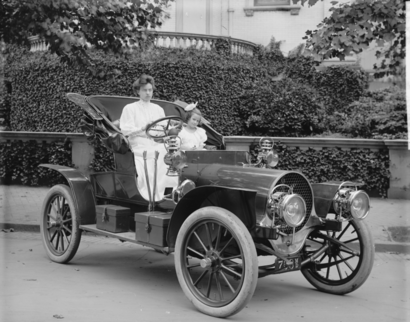
\includegraphics[width=\linewidth]{pic/sample-franklin}
  \caption{1907 Franklin Model D roadster. Photograph by Harris \&
    Ewing, Inc. [Public domain], via Wikimedia
    Commons. (\url{https://goo.gl/VLCRBB}).}\label{fig:franklin}
\end{figure}

Your figures should contain a caption which describes the figure to
the reader. Figure captions are placed \emph{below} the figure.


\section{Citations and Bibliographies}\label{sec:citations}

The use of BibLaTeX for the preparation and formatting of one's
references is strongly recommended. Authors' names should be complete
--- use full first names (``Donald E. Knuth'') not initials
(``D. E. Knuth'') --- and the salient identifying features of a
reference should be included: title, year, volume, number, pages,
article DOI, etc.

The bibliography is included in your source document before 
\texttt{\textbackslash begin\{document\}}:

\texttt{\textbackslash addbibresource\{references.bib\}}

You may change where your bibliography sources are found.

To print the bibliography, issue the command
\texttt{\textbackslash printbibliography[heading=bibintoc]}.
You should set the bibliography to single spacing as well.

\texttt{\{\textbackslash ssp\textbackslash printbibliography[heading=bibintoc]\}}

Citations and references use the author-year style by default. To
enable numeric citations, include \texttt{numcite} as an
option in the document class heading, i.e.:

\texttt{\textbackslash documentclass[numcite]\{nusthesis-neo\}}

Some examples. A normal citation \cite{00}, a parenthesized
citation \parencite{cite:31}, a textual citation \citet{cite:1},
a footnote citation (avoid),\footcite{cite:2} a citation with
prefixes and suffixes \parencite[see][pp. 123--124]{cite:3}, a
citation using natbib-style commands \citep{cite:4}. The
Bib\LaTeX\ cheatsheet\footnote{\url{https://tug.ctan.org/info/biblatex-cheatsheet/biblatex-cheatsheet.pdf}}
contains helpful information for using Bib\LaTeX.

\section{Referencing}
The \texttt{nusthesis-neo} document class includes the \texttt{cleveref}
package for referencing.\footnote{\url{https://ctan.org/pkg/cleveref?lang=en}}
Some examples. \cref{ch:user-guide}, \cref{sec:template-options,sec:typefaces,sec:abstract-name,sec:title},
\cref{sec:subsection}, \cref{sec:subsubsection}, \cref{tab:freq}, \cref{fig:franklin},
\cref{def:no-name}, \cref{lem:named}, \cref{eq:123,eq:33}, \cref{app:moduli} and \cref{app:main-proofs}.

\section{Your Publications}
You may optionally include a list of your publications during your studies
in the appendix. The appendix should be enclosed in the \texttt{refsection}
environment. The publications should be cited within the \texttt{refsection}
environment using \texttt{\textbackslash nocite} so that the citations are
suppressed. Additionally, to highlight your name in the bib entry,
insert the \texttt{me} annotation to your name in the bib entry in the
\texttt{.bib} file.
An example bib entry that highlights ``Jane Tan'' is as follows:

\texttt{@book\{mycitekey, author=\{Lee, Alice and Tan, Jane and Sulaiman, Haikal\}, author+an=\{2=me\}, ...\}}

Note that these highlights will not appear in the original
bibliography list. The name of this appendix can be configured by setting
the \texttt{title} configuration parameter in \texttt{\textbackslash printbibliography}.
See the provided \texttt{chapters/ap-publication.tex} and \texttt{references.bib}
for examples.

\begin{landscape}
\section{Landscape Mode}
The \texttt{nusthesis-neo} document class comes with the \texttt{pdflscape} package.\footnote{\url{https://ctan.org/pkg/pdflscape?lang=en}} To typeset stuff in landscape mode, simply use the \texttt{landscape} environment, as is done for this paragraph. This mode can be used for large, wide figures and tables. Note that the headers and footers remain at the same position and are not rotated, as per NUS requirements.
\end{landscape}
